% Created by tikzDevice version 0.12.6 on 2026-05-14 10:34:49
% !TEX encoding = UTF-8 Unicode
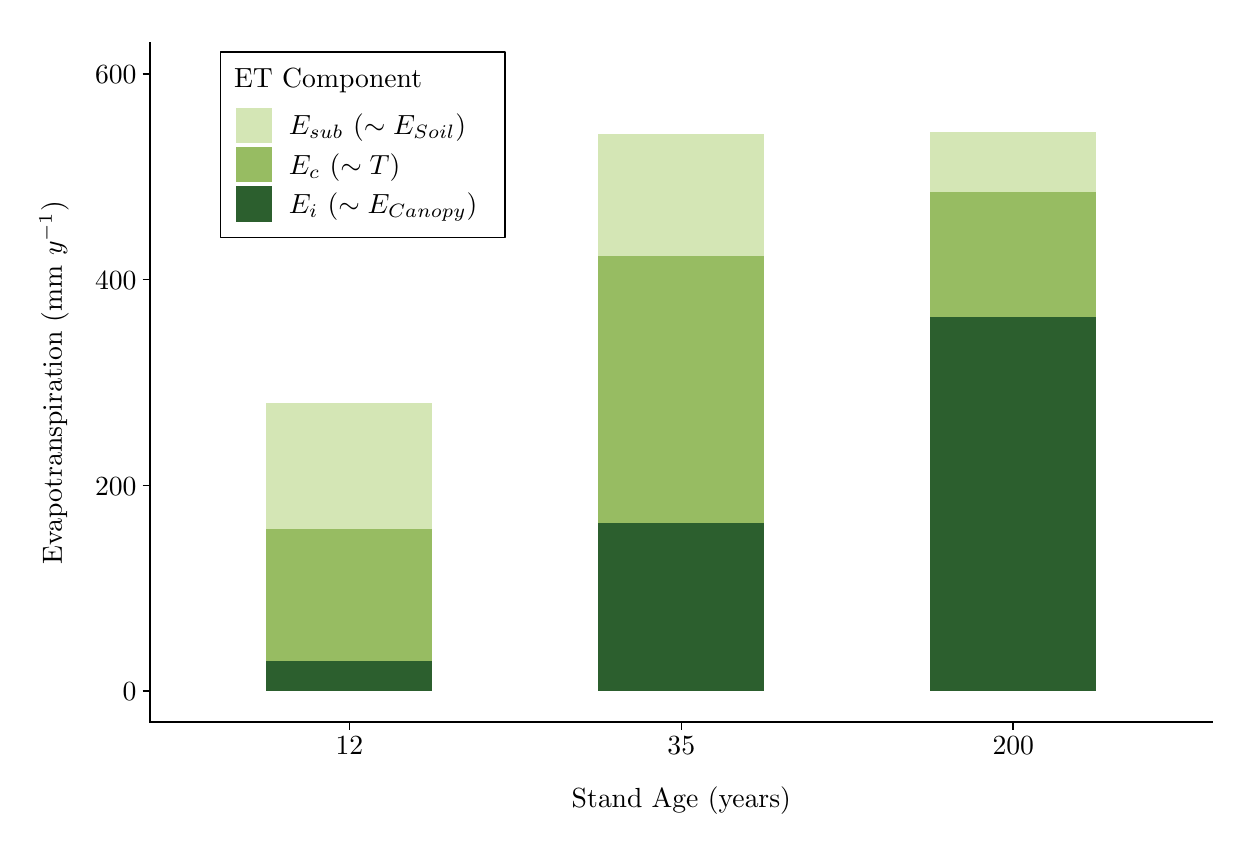
\begin{tikzpicture}[x=1pt,y=1pt]
\definecolor{fillColor}{RGB}{255,255,255}
\path[use as bounding box,fill=fillColor,fill opacity=0.00] (0,0) rectangle (433.62,289.08);
\begin{scope}
\path[clip] (  0.00,  0.00) rectangle (433.62,289.08);
\definecolor{drawColor}{RGB}{255,255,255}
\definecolor{fillColor}{RGB}{255,255,255}

\path[draw=drawColor,line width= 0.6pt,line join=round,line cap=round,fill=fillColor] (  0.00,  0.00) rectangle (433.62,289.08);
\end{scope}
\begin{scope}
\path[clip] ( 44.28, 38.11) rectangle (428.12,283.58);
\definecolor{fillColor}{RGB}{255,255,255}

\path[fill=fillColor] ( 44.28, 38.11) rectangle (428.12,283.58);
\definecolor{fillColor}{RGB}{212,230,181}

\path[fill=fillColor] ( 86.26,108.03) rectangle (146.24,153.41);
\definecolor{fillColor}{RGB}{151,188,98}

\path[fill=fillColor] ( 86.26, 60.06) rectangle (146.24,108.03);
\definecolor{fillColor}{RGB}{44,95,46}

\path[fill=fillColor] ( 86.26, 49.27) rectangle (146.24, 60.06);
\definecolor{fillColor}{RGB}{212,230,181}

\path[fill=fillColor] (206.21,206.59) rectangle (266.19,250.48);
\definecolor{fillColor}{RGB}{151,188,98}

\path[fill=fillColor] (206.21,110.26) rectangle (266.19,206.59);
\definecolor{fillColor}{RGB}{44,95,46}

\path[fill=fillColor] (206.21, 49.27) rectangle (266.19,110.26);
\definecolor{fillColor}{RGB}{212,230,181}

\path[fill=fillColor] (326.16,229.65) rectangle (386.14,251.22);
\definecolor{fillColor}{RGB}{151,188,98}

\path[fill=fillColor] (326.16,184.65) rectangle (386.14,229.65);
\definecolor{fillColor}{RGB}{44,95,46}

\path[fill=fillColor] (326.16, 49.27) rectangle (386.14,184.65);
\end{scope}
\begin{scope}
\path[clip] (  0.00,  0.00) rectangle (433.62,289.08);
\definecolor{drawColor}{RGB}{0,0,0}

\path[draw=drawColor,line width= 0.6pt,line join=round,line cap=rect] ( 44.28, 38.11) --
	( 44.28,283.58);
\end{scope}
\begin{scope}
\path[clip] (  0.00,  0.00) rectangle (433.62,289.08);
\definecolor{drawColor}{RGB}{0,0,0}

\node[text=drawColor,anchor=base east,inner sep=0pt, outer sep=0pt, scale=  1.00] at ( 39.33, 45.83) {0};

\node[text=drawColor,anchor=base east,inner sep=0pt, outer sep=0pt, scale=  1.00] at ( 39.33,120.21) {200};

\node[text=drawColor,anchor=base east,inner sep=0pt, outer sep=0pt, scale=  1.00] at ( 39.33,194.59) {400};

\node[text=drawColor,anchor=base east,inner sep=0pt, outer sep=0pt, scale=  1.00] at ( 39.33,268.98) {600};
\end{scope}
\begin{scope}
\path[clip] (  0.00,  0.00) rectangle (433.62,289.08);
\definecolor{drawColor}{RGB}{0,0,0}

\path[draw=drawColor,line width= 0.6pt,line join=round] ( 41.53, 49.27) --
	( 44.28, 49.27);

\path[draw=drawColor,line width= 0.6pt,line join=round] ( 41.53,123.65) --
	( 44.28,123.65);

\path[draw=drawColor,line width= 0.6pt,line join=round] ( 41.53,198.04) --
	( 44.28,198.04);

\path[draw=drawColor,line width= 0.6pt,line join=round] ( 41.53,272.42) --
	( 44.28,272.42);
\end{scope}
\begin{scope}
\path[clip] (  0.00,  0.00) rectangle (433.62,289.08);
\definecolor{drawColor}{RGB}{0,0,0}

\path[draw=drawColor,line width= 0.6pt,line join=round,line cap=rect] ( 44.28, 38.11) --
	(428.12, 38.11);
\end{scope}
\begin{scope}
\path[clip] (  0.00,  0.00) rectangle (433.62,289.08);
\definecolor{drawColor}{RGB}{0,0,0}

\path[draw=drawColor,line width= 0.6pt,line join=round] (116.25, 35.36) --
	(116.25, 38.11);

\path[draw=drawColor,line width= 0.6pt,line join=round] (236.20, 35.36) --
	(236.20, 38.11);

\path[draw=drawColor,line width= 0.6pt,line join=round] (356.15, 35.36) --
	(356.15, 38.11);
\end{scope}
\begin{scope}
\path[clip] (  0.00,  0.00) rectangle (433.62,289.08);
\definecolor{drawColor}{RGB}{0,0,0}

\node[text=drawColor,anchor=base,inner sep=0pt, outer sep=0pt, scale=  1.00] at (116.25, 26.28) {12};

\node[text=drawColor,anchor=base,inner sep=0pt, outer sep=0pt, scale=  1.00] at (236.20, 26.28) {35};

\node[text=drawColor,anchor=base,inner sep=0pt, outer sep=0pt, scale=  1.00] at (356.15, 26.28) {200};
\end{scope}
\begin{scope}
\path[clip] (  0.00,  0.00) rectangle (433.62,289.08);
\definecolor{drawColor}{RGB}{0,0,0}

\node[text=drawColor,anchor=base,inner sep=0pt, outer sep=0pt, scale=  1.00] at (236.20,  7.44) {Stand Age (years)};
\end{scope}
\begin{scope}
\path[clip] (  0.00,  0.00) rectangle (433.62,289.08);
\definecolor{drawColor}{RGB}{0,0,0}

\node[text=drawColor,rotate= 90.00,anchor=base,inner sep=0pt, outer sep=0pt, scale=  1.00] at ( 12.39,160.85) {Evapotranspiration (mm $y^{-1}$)};
\end{scope}
\begin{scope}
\path[clip] (  0.00,  0.00) rectangle (433.62,289.08);
\definecolor{drawColor}{RGB}{0,0,0}
\definecolor{fillColor}{RGB}{255,255,255}

\path[draw=drawColor,line width= 0.5pt,line join=round,line cap=round,fill=fillColor] ( 69.61,213.25) rectangle (172.48,280.27);
\end{scope}
\begin{scope}
\path[clip] (  0.00,  0.00) rectangle (433.62,289.08);
\definecolor{drawColor}{RGB}{0,0,0}

\node[text=drawColor,anchor=base west,inner sep=0pt, outer sep=0pt, scale=  1.00] at ( 74.61,267.41) {ET Component};
\end{scope}
\begin{scope}
\path[clip] (  0.00,  0.00) rectangle (433.62,289.08);
\definecolor{fillColor}{RGB}{255,255,255}

\path[fill=fillColor] ( 74.61,246.71) rectangle ( 88.84,260.93);
\definecolor{fillColor}{RGB}{212,230,181}

\path[fill=fillColor] ( 75.32,247.42) rectangle ( 88.13,260.22);
\end{scope}
\begin{scope}
\path[clip] (  0.00,  0.00) rectangle (433.62,289.08);
\definecolor{fillColor}{RGB}{255,255,255}

\path[fill=fillColor] ( 74.61,232.48) rectangle ( 88.84,246.71);
\definecolor{fillColor}{RGB}{151,188,98}

\path[fill=fillColor] ( 75.32,233.19) rectangle ( 88.13,246.00);
\end{scope}
\begin{scope}
\path[clip] (  0.00,  0.00) rectangle (433.62,289.08);
\definecolor{fillColor}{RGB}{255,255,255}

\path[fill=fillColor] ( 74.61,218.25) rectangle ( 88.84,232.48);
\definecolor{fillColor}{RGB}{44,95,46}

\path[fill=fillColor] ( 75.32,218.97) rectangle ( 88.13,231.77);
\end{scope}
\begin{scope}
\path[clip] (  0.00,  0.00) rectangle (433.62,289.08);
\definecolor{drawColor}{RGB}{0,0,0}

\node[text=drawColor,anchor=base west,inner sep=0pt, outer sep=0pt, scale=  1.00] at ( 94.34,250.38) {$E_{sub}$ ($\sim E_{Soil})$};
\end{scope}
\begin{scope}
\path[clip] (  0.00,  0.00) rectangle (433.62,289.08);
\definecolor{drawColor}{RGB}{0,0,0}

\node[text=drawColor,anchor=base west,inner sep=0pt, outer sep=0pt, scale=  1.00] at ( 94.34,236.15) {$E_c$ ($\sim T)$};
\end{scope}
\begin{scope}
\path[clip] (  0.00,  0.00) rectangle (433.62,289.08);
\definecolor{drawColor}{RGB}{0,0,0}

\node[text=drawColor,anchor=base west,inner sep=0pt, outer sep=0pt, scale=  1.00] at ( 94.34,221.92) {$E_i$ ($\sim E_{Canopy})$};
\end{scope}
\end{tikzpicture}
